%% Ankur Sinha

%% packages %%
% support for coloured text
\usepackage{color}
% IPA
\usepackage{tipa}
\usepackage[scale=2]{ccicons}
\usepackage{amssymb}
\usepackage{tikz}
\usetikzlibrary{mindmap, arrows.meta, positioning, arrows}
\usepackage{pgfplots}
% Define the colours we use for E and I in all graphs
\definecolor{SinhaBlueE}{HTML}{3b4cc0}
\definecolor{SinhaRedI}{HTML}{f7a789}
\pgfmathdeclarefunction{gaussnew}{4}{%nu, eta, eps, omega
  \pgfmathparse{(#1*((2*exp(-(((x-((#2+#3)/2))/((#2-#3)/(2*sqrt(-ln(#4/2)))))^2))) -#4))}%chktex 36
}
\usepackage{jneurosci}
\usepackage{subcaption}
\usepackage[T1]{fontenc}
\usepackage[utf8]{inputenc}
\usepackage[style=nature,backend=biber,autocite=footnote]{biblatex}
\addbibresource{masterbib.bib}
\renewcommand*{\bibfont}{\tiny}
% Use opensans
% \usepackage[default,scale=0.95]{opensans}
\usepackage[sfdefault]{roboto}
% for strike through
\usepackage[normalem]{ulem}
% links, urls, refs
\definecolor{links}{HTML}{2A1B81}
% Fedora blue for the theme
\definecolor{FedoraBlue}{HTML}{2A1B81}
\usepackage{hyperref}
\hypersetup{colorlinks,linkcolor=Green,urlcolor=links}
% graphics
\usepackage{graphicx}
% algorithm
\usepackage{algorithmic}
\usepackage{textcomp}
\usepackage{wrapfig}
\usepackage{textgreek}
\usepackage{euler}
\usepackage{csquotes}
\usepackage{tabularx}
\usepackage{booktabs}
% beamer theme
% use defaults for theme
\usetheme[numbering=fraction]{metropolis}
\usefonttheme[onlymath]{serif}
\setbeamerfont{footnote}{size=\tiny}
\setbeamerfont{caption}{size=\tiny}
\setbeamercolor{alerted text}{fg=Green}
\setbeamerfont{note page}{size=\small}

% Not needed in metropolis, but in general footnote citation fixes: https://tex.stackexchange.com/questions/44217/how-can-i-stop-footcite-from-hijacking-my-beamer-columns
% how to use multiple references to the same footnote: https://tex.stackexchange.com/questions/27763/beamer-multiple-references-to-the-same-footnote

% Disable footnoterule
\renewcommand{\footnoterule}{}

%% title %%
\title{Associative memory performance in peripherally-lesioned networks repaired by homeostatic structural plasticity}
\subtitle{CNS*2020: P195}
\author[Ankur Sinha]{Ankur Sinha*, Christoph Metzner, Rod Adams, Neil Davey, \\Michael Schmuker, and Volker Steuber\\UH Biocomputation Group, Hatfield UK.}
\date{19/07/2020}

%% document begins %%
\begin{document}


% title frame %%
\begin{frame}
  \titlepage{}
\end{frame}

%% Three slides for 5 minutes seems good
%% So, 30 slides at most for 50 minutes
\begin{frame}[c]
  \frametitle{Research question}
  How does repair by structural plasticity affect the recall performance of associative memory stored in an balanced cortical network after focal peripheral lesions?
\end{frame}
\begin{frame}[c]
  \frametitle{New model of peripheral lesioning and repair in cortical network}
  \begin{figure}[h]
    \centering
    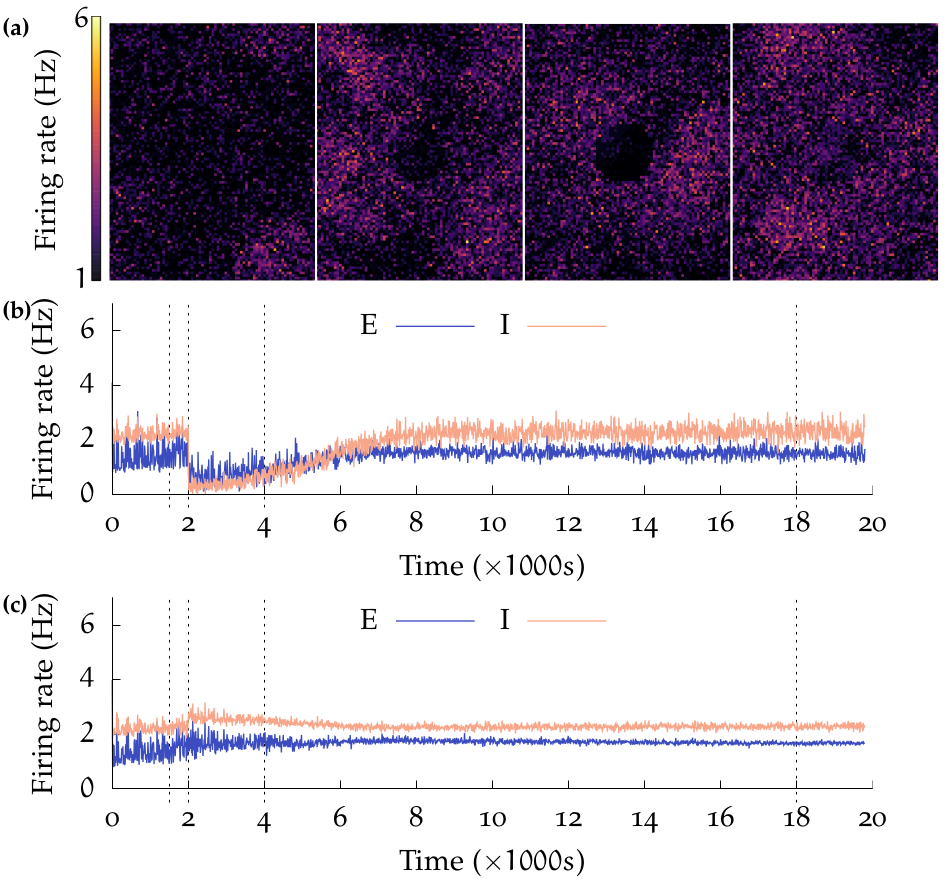
\includegraphics[width=0.5\linewidth]{99_images/deaff-repair}
    \caption{\textbf{(a)} firing rates of the network at different points of time in the simulation. As can be seen in panel 4, activity is restored to deprived neurons in the central Lesion Projection Zone (LPZ).
      \textbf{(b)} mean firing rates of neurons in the centre of the LPZ over time.
      \textbf{(c)} mean firing rates of neurons on the outer periphery of the LPZ over time. 
      The dashed lines in (b) and (c) correspond to the panels in (a).}
  \end{figure}
  \footnotetext[1]{Manuscript in review, preprint: \fullcite{Sinha2019}}
\end{frame}
\begin{frame}[c]
  \frametitle{Model overview}
  \begin{figure}[h]
    \centering
    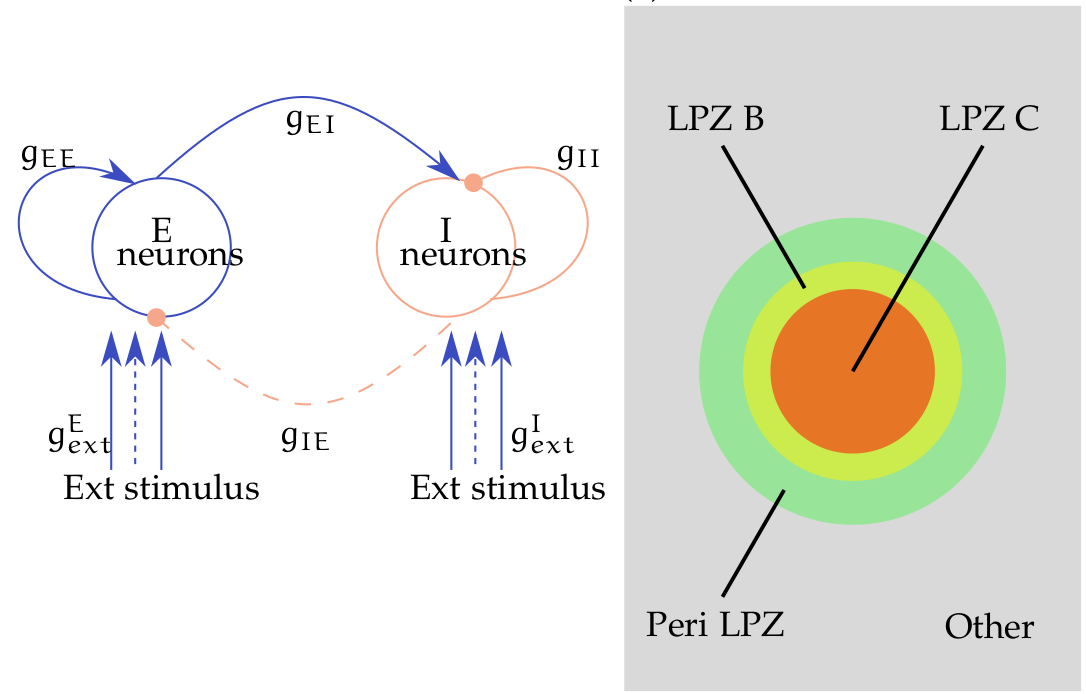
\includegraphics[width=0.6\linewidth]{99_images/schematic}
    \caption{The network consists of excitatory and inhibitory conductance based point neurons connected recurrently, and distributed in a 2D plane. Inhibitory synaptic plasticity\footnotemark[2]{} modulates the efficacy of IE synapses, while all other synapses are static. Structural plasticity\footnotemark[3]{} acts on all recurrent synapses in the network. To model  peripheral lesion, external input is removed from a set of neurons in the centre of the plane to form the Lesion Projection Zone (LPZ). For analysis, the LPZ is divided into 4 sub-regions, the centre of the LPZ (LPZ C), the inner border (LPZ B), the outer periphery (peri-LPZ), and the remaining neurons.}
  \end{figure}%
  \footnotetext[2]{\fullcite{Vogels2011}}
  \footnotetext[3]{\fullcite{Butz2013}}
\end{frame}
\begin{frame}[c]
  \frametitle{Simulation protocol}
  \begin{figure}[h]
    \centering
    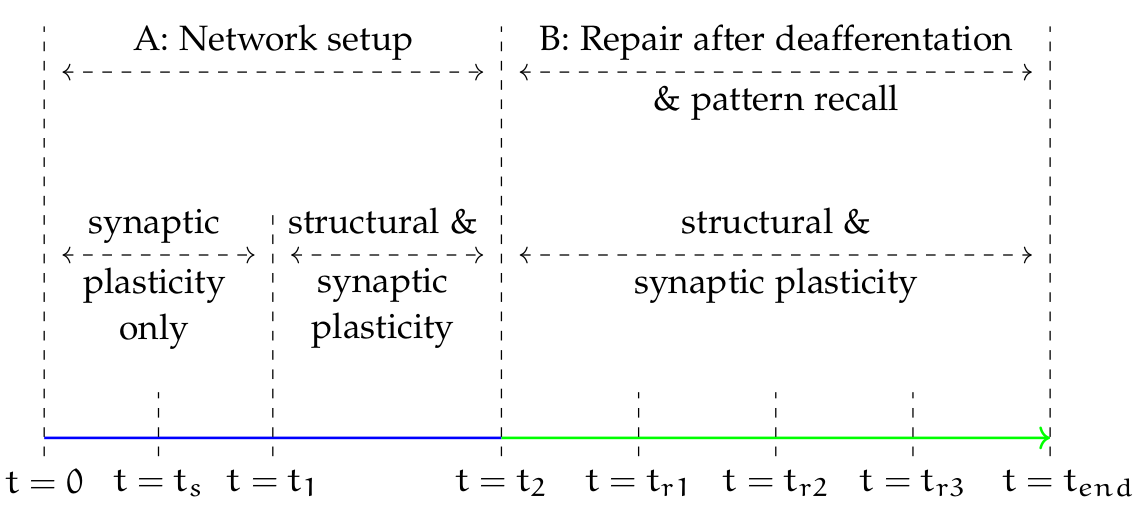
\includegraphics[width=0.8\linewidth]{99_images/recall-protocol}
    \caption{The network is set up with its initial connectivity and allowed to stabilise to its AI regime. Then, at \(t_s\), an associative memory is stored by strengthening the synapses between a randomly selected set of neurons. The network is again allowed to re-stabilise to its AI state. If needed, more patterns are stored in the network in this way. When the last associative memory has been stored and the network returned to its balanced state a snapshot of the network is saved. Then, the stored associative memories are recalled by providing stimulus to a subset of the neurons forming each pattern. The firing rates of the neurons in the associative memory, forming the pattern, and the rest of the neurons of the population, which form the background, allow the calculation of the SNR\@.}%
  \end{figure}
\end{frame}
\begin{frame}[c]
  \frametitle{Associative memory performance drops after deafferentation}
  \begin{figure}[h]
    \centering
    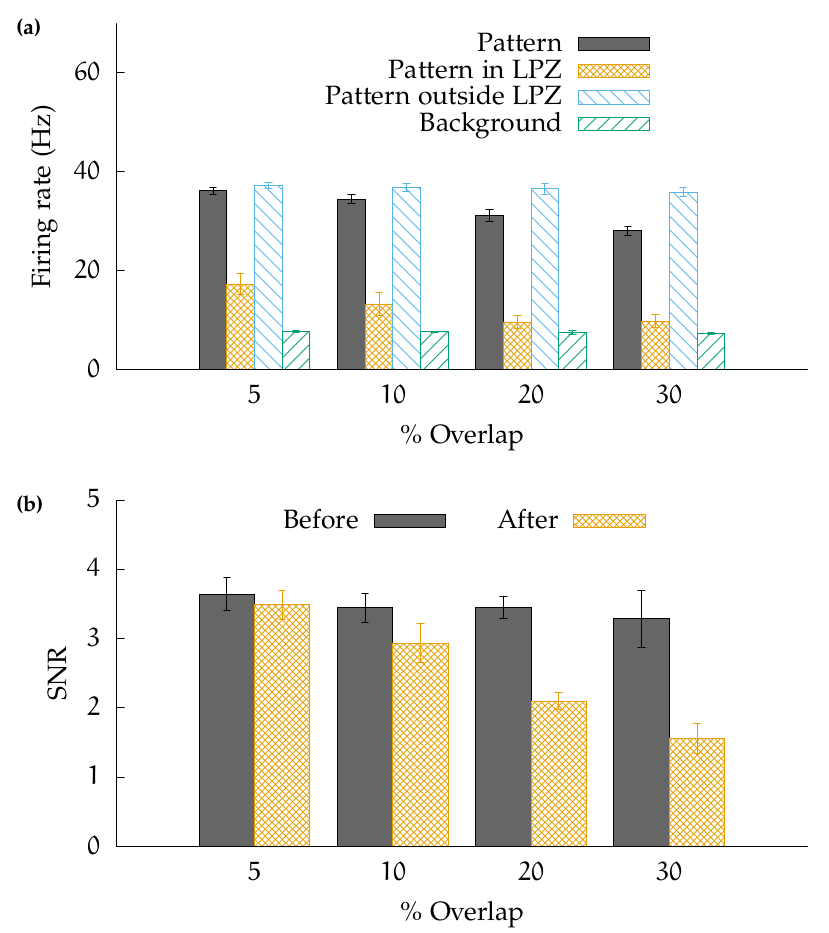
\includegraphics[width=0.55\linewidth]{99_images/performance-deaff-only}
    \caption{Performance of associative memory recall for varying amounts of the pattern falling in the LPZ (\% Overlap). \textbf{(a)} population firing rates; \textbf{(b)} SNR\@.}
  \end{figure}
\end{frame}
\begin{frame}[c]
  \frametitle{Associative memory performance is not restored by repair}
  \begin{figure}[h]
    \centering
    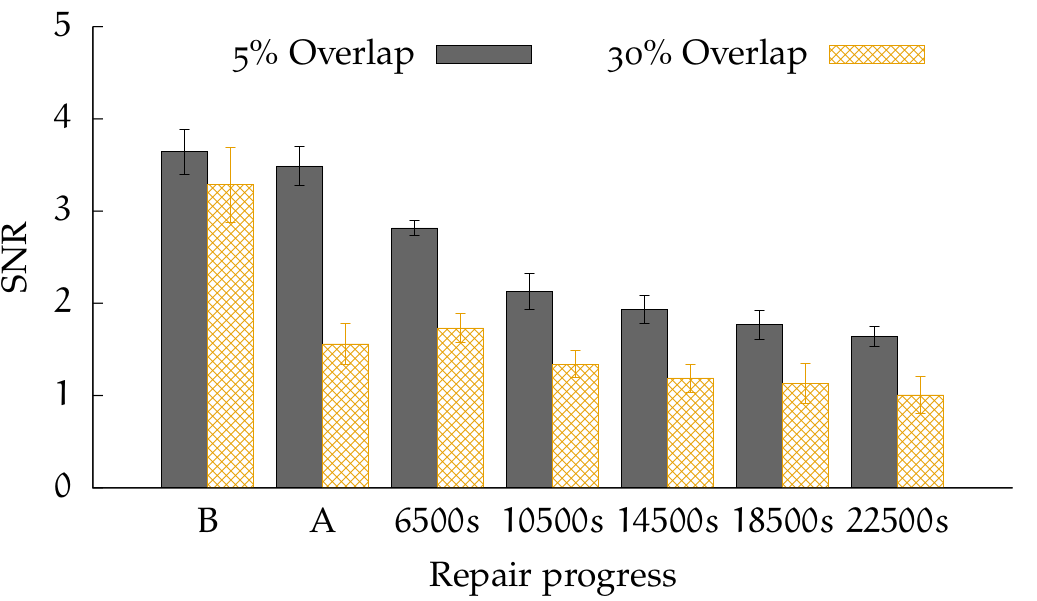
\includegraphics[width=0.6\linewidth]{99_images/performance-during-repair}
    \caption{SNR during memory recall before (B) and after (A) deafferentation, and during the repair by structural plasticity for different levels of overlap.}
  \end{figure}
\end{frame}
\begin{frame}[c]
  \frametitle{Conclusions}
  While average activity is restored to the network by structural plasticity after deafferentation, \alert{performance of associative memory is not restored}.
\end{frame}
\begin{frame}[c]
  \frametitle{Open questions for future work}
  \begin{itemize}
    \item Experimental validation of peripheral lesioning model\footnotemark[4]{}.
    \pause{}
    \item Should performance be retained after deprivation by peripheral lesions?
      \pause{}
    \item How can the performance be retained/improved?
      \begin{itemize}
        \item Modulation of the structural plasticity process?
        \item Retraining/recall of associative memory during repair?
      \end{itemize}
      \pause{}
    \item If performance is not retained, does the network continue to function as an associative memory store for new memories?
  \end{itemize}
  \footnotetext[4]{Manuscript in review, preprint: \fullcite{Sinha2019}}
\end{frame}
\begin{frame}[t,allowframebreaks]
  \frametitle{Bibliography}
  \printbibliography[heading=none]{}
\end{frame}
\end{document}

